\section{Localization and the chord mean}\label{c7:localization}

The cylinder estimate bounds the total weight of incompatible pairs of
separating cycles. We use that bound to remove cycles that travel far
from the mark they enclose. We compare the remaining cycles with two
planar nesting partitions, one near each mark. This gives the planar nesting
exponent and completes the chord-length calculation.

Use the balanced physical cylinder with period
\[
 P=(M,0),\qquad M=2m,\qquad m\ \text{even},
\]
and marked tessellation vertices \(O=(0,0)\) and \(O'=(M/2,0)\).
For a separating cycle \(\lambda\), write
\(w_\lambda=x^{|\lambda|}\). Two cycles are incompatible when they
share a honeycomb vertex; in particular, a cycle is incompatible with
itself. Expanding the positive cylinder partition at \(g=0\) gives
\[
 I_M:=\sum_{\substack{\lambda,\lambda'\ {\rm separating}\\
                 \lambda,\lambda'\ {\rm incompatible}}}
          w_\lambda w_{\lambda'}
   =-\left.\partial_g^2\log G_{A,B}(g)\right|_{g=0}
   =O(\log M).
\]
The pairs in this sum are ordered. Indeed the square of the linear
coefficient counts every ordered pair, whereas twice the quadratic
coefficient counts exactly the ordered compatible pairs.

We first record the separation facts used below. A contractible simple
cycle on the cylinder bounds a unique embedded closed disk. If the cycle
separates \(O\) and \(O'\), this disk contains exactly one of them.
Choose its planar lift containing the specified lift of that mark. Two
disjoint contractible boundaries have disks that are either disjoint or
strictly nested, by Jordan separation. Hence disjoint same-mark
boundaries have strictly nested disks, while disjoint opposite-mark
boundaries have disjoint disks. These alternatives hold literally for
the chosen lifts: a lift of an embedded disk cannot contain two period
translates of a mark. Finally, strict containment of compact disks
implies strict inequality of their Euclidean diameters. To see this,
extend one endpoint of a diameter-realizing pair a short distance inside
the outer disk.

\begin{lemma}[Cycles escaping the two marks]\label{j:localization-escape}
Fix \(C>1\). For a contractible separating cycle, measure horizontal
coordinates relative to the enclosed mark in its chosen disk lift.
Let \(\mathcal E_M\) consist of all noncontractible separating cycles
and all contractible separating cycles whose chosen disk either reaches
\(|x_{\rm horiz}|\ge M/4\) or has diameter greater than \(CM\).
Then
\[
 \sum_{\lambda\in\mathcal E_M}w_\lambda
 \le (5\sqrt2+2)\sqrt{I_M}.
\]
Every cycle outside \(\mathcal E_M\) has a disk lift contained in the
closed Euclidean ball of radius \(CM\) about its enclosed mark.
\end{lemma}

\begin{proof}
All class sums may first be restricted to finite subfamilies; monotone
convergence then gives the stated bounds and their finiteness.

First consider disks enclosing \(O\), with lifts containing the origin.
Call a disk \emph{wide} if it reaches \(|x_{\rm horiz}|\ge M/4\), and
write \(S_W\) for the total weight of their boundaries. Let \(V^*\) be
the reflection of \(V\) in the vertical axis, and put \(t=(M/2,0)\).
Reflection fixes both cylinder marks, and translation by \(t\)
interchanges them. Both operations preserve the honeycomb graph and
give weight-preserving injections on these cycles.

Suppose \(U,V\) are wide and
\(\operatorname{diam}U\ge\operatorname{diam}V\). If the boundary of
\(U\) were compatible with the boundaries of both \(V\) and \(V^*\), the same-mark
alternatives above and the diameter ordering would give
\[
 V\cup V^*\subset\operatorname{int}U.
\]
Compatibility also with the boundaries of \(V+t\) and \(V^*+t\) would make those
opposite-mark disks disjoint from \(U\). These conclusions conflict.
In fact, a path in \(V\) from the origin to a wide point meets one of
the lines \(x_{\rm horiz}=\pm M/4\), say at \(p_+\) or \(p_-\).
Reflection supplies the other point at the same height. Thus
\[
 p_-\in V\cup V^*,\qquad
 p_+=p_-+t\in V\cup V^*,
\]
so \(V\cup V^*\) meets \((V\cup V^*)+t\). This uses only a path in the
disk, not convexity or connectedness of any horizontal slice.
Figure~\ref{j:fig-localization}(a) shows this contact.

For each diameter-sorted pair, at least one of the four indicated
images is therefore incompatible with \(U\). Each image map is
injective and preserves weight, so each of the four sums is at most
\(I_M\). The diameter-sorted pairs carry at least half of \(S_W^2\).
Consequently
\[
 \frac12S_W^2\le4I_M,\qquad S_W\le\sqrt{8I_M}.
\]

\begin{figure}[ht]
\centering
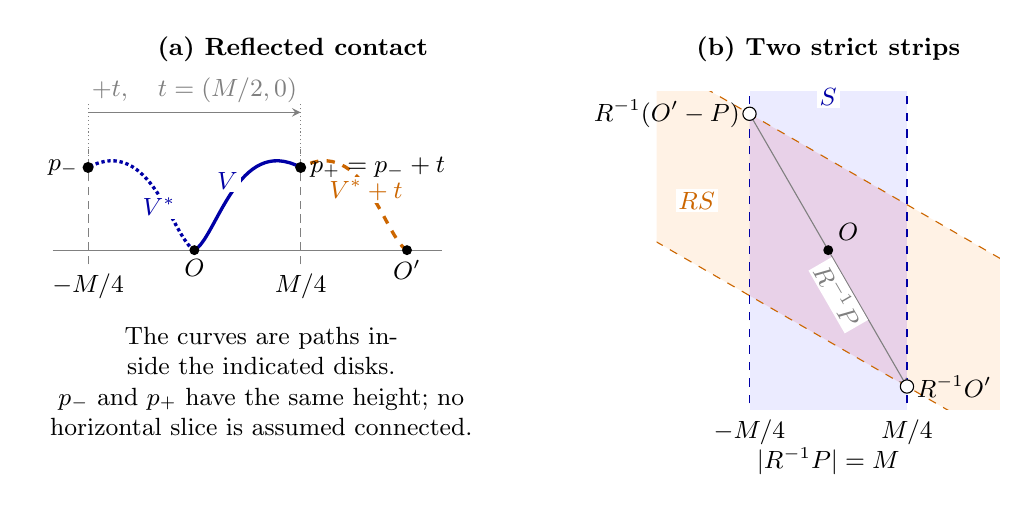
\begin{tikzpicture}[x=1cm,y=1cm,>=stealth,font=\small]
 \begin{scope}[shift={(2.4,0)}]
  \node[font=\small\bfseries] at (1.25,2.55) {(a) Reflected contact};
  \draw[gray] (-1.8,0)--(3.15,0);
  \draw[densely dashed,gray] (-1.35,-.18)--(-1.35,1.28);
  \draw[densely dashed,gray] (1.35,-.18)--(1.35,1.28);
  \draw[very thick,blue!65!black]
    (0,0) .. controls (.28,.15) and (.55,1.48) .. (1.35,1.05);
  \draw[very thick,blue!65!black,densely dotted]
    (0,0) .. controls (-.28,.15) and (-.55,1.48) .. (-1.35,1.05);
  \draw[very thick,orange!80!black,dashed]
    (2.7,0) .. controls (2.42,.15) and (2.15,1.48) .. (1.35,1.05);
  \draw[densely dotted,gray] (-1.35,1.05)--(-1.35,1.85);
  \draw[densely dotted,gray] (1.35,1.05)--(1.35,1.85);
  \draw[->,gray] (-1.35,1.75)--(1.35,1.75)
    node[midway,above] {$+t,\quad t=(M/2,0)$};
  \fill (0,0) circle (1.8pt) node[below] {$O$};
  \fill (2.7,0) circle (1.8pt) node[below] {$O'$};
  \fill (-1.35,1.05) circle (2pt)
    node[left] {$p_-$};
  \fill (1.35,1.05) circle (2pt)
    node[right] {$p_+=p_-+t$};
  \node[below] at (-1.35,-.18) {$-M/4$};
  \node[below] at (1.35,-.18) {$M/4$};
  \node[blue!65!black,fill=white,inner sep=1pt] at (.42,.88) {$V$};
  \node[blue!65!black,fill=white,inner sep=1pt] at (-.45,.55) {$V^*$};
  \node[orange!80!black,fill=white,inner sep=1pt] at (2.18,.76) {$V^*+t$};
  \node[anchor=north,align=center,text width=5.7cm] at (.85,-.85)
    {The curves are paths inside the indicated disks.\\
     \(p_-\) and \(p_+\) have the same height; no horizontal
     slice is assumed connected.};
 \end{scope}
 \begin{scope}[shift={(10.45,0)}]
  \node[font=\small\bfseries] at (0,2.55) {(b) Two strict strips};
  \begin{scope}
   \clip (-2.18,-2.02) rectangle (2.18,2.02);
   \fill[blue!8] (-1,-3) rectangle (1,3);
   \begin{scope}[rotate=60]
    \fill[orange!10] (-1,-3) rectangle (1,3);
   \end{scope}
   \fill[violet!18]
     (1,.57735)--(1,-1.73205)--(-1,-.57735)--(-1,1.73205)--cycle;
   \draw[blue!65!black,dashed] (-1,-3)--(-1,3);
   \draw[blue!65!black,dashed] (1,-3)--(1,3);
   \begin{scope}[rotate=60]
    \draw[orange!80!black,dashed] (-1,-3)--(-1,3);
    \draw[orange!80!black,dashed] (1,-3)--(1,3);
   \end{scope}
  \end{scope}
  \draw[->,gray] (-1,1.73205)--(1,-1.73205)
    node[pos=.64,sloped,below,fill=white,inner sep=1pt] {$R^{-1}P$};
  \fill (0,0) circle (1.8pt) node[above right] {$O$};
  \draw[fill=white] (-1,1.73205) circle (2.4pt)
    node[left] {$R^{-1}(O'-P)$};
  \draw[fill=white] (1,-1.73205) circle (2.4pt)
    node[right] {$R^{-1}O'$};
  \node[blue!65!black,fill=white,inner sep=1pt] at (0,1.95) {$S$};
  \node[orange!80!black,fill=white,inner sep=1pt] at (-1.67,.63) {$RS$};
  \node[below] at (-1,-2.03) {$-M/4$};
  \node[below] at (1,-2.03) {$M/4$};
  \node at (0,-2.68) {$|R^{-1}P|=M$};
 \end{scope}
\end{tikzpicture}

\caption{The two planar constructions in the escape bound.
In (a), only connecting paths inside \(V\), \(V^*\), and \(V^*+t\)
are drawn; the two marked points at a common height establish the contact without
asserting that a horizontal slice is connected. In (b),
\(S=\{|x_{\rm horiz}|<M/4\}\) and \(RS\) are the two open strips.
The open circles are adjacent rotated-back lifts of the opposite mark.
Their separation is \(M\), the long diagonal of the strip intersection.
The paths in (a) are schematic; (b) is drawn to scale.}\label{j:fig-localization}
\end{figure}

Now let \(U\) be nonwide and have diameter greater than \(CM\). It is
contained in the strict strip \(S=\{|x_{\rm horiz}|<M/4\}\). Let \(R\)
be rotation by \(\pi/3\) about \(O\). Although this rotation is not an
automorphism of the cylinder, \(RU\) projects to an embedded disk on
the same cylinder. Indeed
\[
 R^{-1}P=(M/2,-\sqrt3M/2),
\]
and the strips \(S\) and \(S+kR^{-1}P\) are disjoint for every nonzero
integer \(k\). Hence \(RU\) is disjoint from all its nontrivial period
translates. Moreover
\[
 \bigl(R^{-1}(O'+kP)\bigr)_{\rm horiz}=M/4+kM/2
\]
lies outside \(S\) for every integer \(k\). The projected disk therefore
encloses \(O\) and excludes \(O'\). Rotation preserves the honeycomb
graph and the weight. It is injective on this class because the image
disk has a unique lift containing the origin.

For any two such disks \(U,V\), compatibility of the boundaries of
\(U\) and \(RV\) would force one disk strictly inside the other.
The inner disk would then lie in \(S\cap RS\). The closure of this
intersection is a parallelogram with diagonals \(M\) and \(M/\sqrt3\);
in particular its diameter is \(M\), as shown in
Figure~\ref{j:fig-localization}(b). Both candidate inner disks have
diameter greater than \(CM>M\), a contradiction. Every original/image
pair is incompatible, so the weight \(S_L\) of this nonwide large class
satisfies
\[
 S_L^2\le I_M.
\]
Translation by \(t\) gives the identical two estimates for disks
enclosing \(O'\).

It remains to handle noncontractible cycles. Each simple
noncontractible cycle separates the two ends of the infinite cylinder.
Two disjoint such cycles are vertically ordered: after compactifying
the two ends, this is the nesting order of two disjoint curves
separating the two added points. Divide the cycles that separate the
marks into two classes according as \(O\) lies in their upper or lower
component. A cycle in one class is incompatible with every cycle in
the other, since disjoint vertically ordered cycles cannot reverse the
order of \(O,O'\). Reflection in the horizontal line interchanges the
classes and preserves weight. If each class has weight \(s\), their
ordered cross-pairs give \(I_M\ge2s^2\). Their combined weight is
therefore at most \(\sqrt{2I_M}\).

The two wide classes, the two nonwide large classes, and the
noncontractible classes are disjoint and exhaust \(\mathcal E_M\).
Their bounds sum to
\[
 2\sqrt{8I_M}+2\sqrt{I_M}+\sqrt{2I_M}
   =(5\sqrt2+2)\sqrt{I_M}.
\]
Outside these classes a disk contains its marked lift and has diameter
at most \(CM\), so every point in it is within distance \(CM\) of that
mark.
\end{proof}

We now compare the cylinder partition with \(\mathcal Z\), the planar
\(+2\) nesting partition defined in Section~\ref{c7:boundary}.
At fugacity \(2\), dropping every disjointness constraint involving
\(\mathcal E_M\) costs at most
\[
 \prod_{\lambda\in\mathcal E_M}(1+2w_\lambda)
 \le \exp\left(2\sum_{\lambda\in\mathcal E_M}w_\lambda\right)
 =\exp(O(\sqrt{\log M})).
\]
Every remaining disk lift lies in a ball of radius \(CM\). A regular
tessellation hexagon of side \(\lceil C'M\rceil\), for fixed
\(C'>2C/\sqrt3\), contains this ball. Same-mark disjointness is
preserved on the chosen lifts. Dropping constraints between the two
marks therefore bounds the remaining partition by the product of the
two corresponding planar partitions.

For the reverse comparison fix \(0<c<1/4\). Hexagons of side
\(\lfloor cM\rfloor\) about the two marked lifts, together with all
their period translates, are pairwise disjoint for large \(M\).
Their surrounding cycles project to separating cylinder cycles with
all joint disjointness preserved. We have proved
\[
 \mathcal Z(\lfloor cM\rfloor)^2
 \le G_{A,B}(2)
 \le \mathcal Z(\lceil C'M\rceil)^2
       \exp(O(\sqrt{\log M})).
\]
The cylinder estimate \(G_{A,B}(2)=M^{1/6+o(1)}\) now gives
\(\mathcal Z(R)=R^{1/12+o(1)}\). To pass from the displayed arguments
to every integer \(R\), use monotonicity of \(\mathcal Z\). For its upper
bound choose the least multiple \(M\) of \(4\) with
\(\lfloor cM\rfloor\ge R\); for its lower bound choose the greatest
multiple \(M\) of \(4\) with \(\lceil C'M\rceil\le R\).
These choices differ from \(R/c\) and \(R/C'\), respectively, by
bounded additive amounts.

Substituting this nesting exponent in the bounds for the mean in
Section~\ref{c7:boundary} gives
\[
 \mathbb E_R^{\rm chord}N=R^{4/3+o(1)}.
\]
For the bulk-visit conclusion, Proposition~\ref{j:visit} compares the
ordinary visit mass with \(\sum_{f\sim v}Z_D(f)\) by
\eqref{j:visit-identity} and \eqref{j:incident-face-partition}.
The domain inclusions following that proposition therefore give,
uniformly for honeycomb vertices \(v\) at distance at most \(R/10\)
from the center,
\[
 c\mathcal Z(\lfloor R/2\rfloor)
 \le \mathcal V_R(v)\le C\mathcal Z(3R)
\]
for all sufficiently large integer \(R\). Using the chord normalization
\eqref{j:chord-partition}, we obtain
\[
 \mathbb P_R^{\rm chord}(v\in\gamma)
   =\frac{\mathcal V_R(v)}{Z_R^{\rm chord}}
   =R^{-2/3+o(1)}
\]
uniformly in the stated range. This proves the mean and bulk-visit
conclusions of Theorem~\ref{j:hexagon}.
